\chapter{Design and Implementation}
\label{chapter: Design and implementation}
The content of the following chapter is about the dataset source description and the images' origin of dermatological characteristic. Further on, the text indicates the \textbf{data pre-processing} procedures in order to re-scale the original images as well as normalizing the labels that identify the skin diseases,  besides the augmentation on data processing. 

Another section forming this chapter is the\textbf{ implementation} of a Convolutional Neural Network based on \textit{EfficientNe}t architecture and pre-trained with \textit{Imagenet} dataset. This neural network will be trained with a small selection of data to obtain appropriate metrics using fine-tuning parameters.

Based on the previously mentioned architecture, different neural networks will be built, trained, and tested. Meanwhile, their scores will be reviewed in the next chapter. 

%%% SECTION

\section{Dataset description}

\begin{wrapfigure}{r}{0.45\textwidth} 
    \vspace{-20pt}
    \centering
        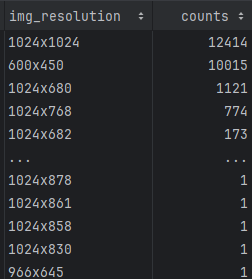
\includegraphics[scale=0.75 ]{images/Building/resolution_list.png}
        \caption{Images resolution distribution Spreadsheet.}
    \label{fig:Spreadsheet_resolution_images}
    \vspace{-100pt}
\end{wrapfigure}

In this section, the \textit{ISIC Challenge dataset}  2019 was used.  It is formed by a set of 25,331 dermoscopic images related to 8 different types of skin diseases \cite{dataset_ref_1}, \cite{dataset_ref_2} y \cite{dataset_ref_3}. The images are stored in \textbf{various resolution sizes that need to be unified into a smaller single-size}. A representation of the image resolution is given in the following table \ref{fig:Spreadsheet_resolution_images}. 

\newpage
As these are real patient images, we also encounter other shapes and features such as hair, lesion markers and other objects that can distort the sample.

The dataset used for this research implies a larger quantity of one specific kind of images that causes an imbalance concerning the proportion of the total images quantity in each class, being Nevus the one with the biggest class with more than 10.000 images. This compared with DF only having 215 images, causes an enormous disparity. Figure \ref{fig:class_distribution_for_train} shows how the different classes are distributed across the dataset. 

\begin{figure}[ht]
    \centering
        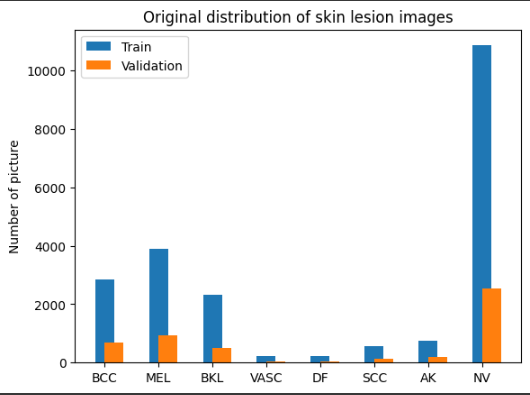
\includegraphics[scale=0.75]{images/Building/Original_distribution_skin_lesion_images.png}
        \caption{Original class distribution for training.}
    \label{fig:class_distribution_for_train}
\end{figure}


A disproportioned dataset could result in wrong output metrics because there is an induced bias during the network training, this might cause the network to give more importance to those classes with more weight in the dataset distribution. As a result, the lower weight classes could be ignored affecting the neural network performance. Due to all this, it is necessary to balance the dataset prior to training the neural network, so that every dataset class has the same weight, improving the network capability to learn. 

Different techniques to correct an unbalanced dataset exist, such as: 
\begin{enumerate}
    \item \textbf{Re-sampling Techniques}: Consists of applying oversampling or sub-sampling in order to make equal class proportions.    
    \item \textbf{Data augmentation}: Involves doing different copies of a picture introducing variables such as picture proportion, brightness, colour saturation and others.
    \item \textbf{Feature selection}: Includes a careful selection of the main feature that describes the image to improve the minority classes' representation.
    \item \textbf{Sintetic image generation}: This technique involves the creation of artificial images that are very similar to the real thing.  

\end{enumerate}



     
%% Data Preparation
\section{Data Preparation}
Neural networks process data in matrix format.  The size of the dataset downloaded from ISIC exceeds 2 GB information in image format. This makes it difficult to handle as a whole. In addition, as we have seen above, these images have different resolutions and an imbalance between the different classes \ref{fig:class_distribution_for_train}. The high level of processing required to convert the original resolution images into matrix numbers is shown in \ref{fig: Data preparation steps}. This one is composed of three steps that will be explained as follows:

\begin{figure}[ht]
    \begin{center}
        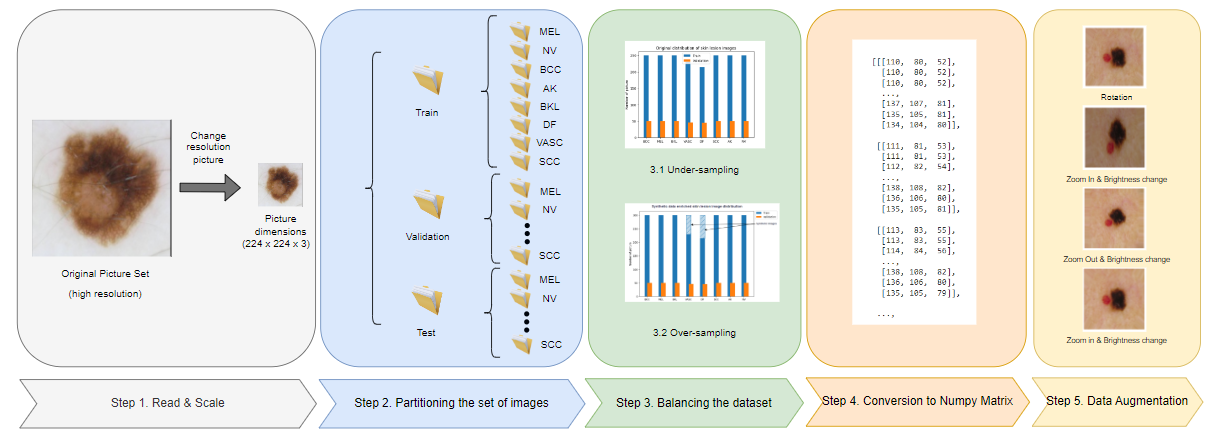
\includegraphics[scale=0.5]{images/Data_Preparation/TFM_DataPreparation_Image.png}
        \caption{xxxxx.}
    \label{fig: Data preparation steps}    
    \end{center}
\end{figure}

\textbf{Step 1. Changing image resolution}
As we introduced in the previous chapter, images came originally in a wide variety of resolutions. According to that, it will be necessary to reduce and reshape them. So as to, make them to be the same resolution and square-shaped . The size is determined by the network used as the feature extractor. In this work, we will use EfficenteNet B0, which requires an input size (224x244x3) corresponding to the width, height and number of channels of the image.

\textbf{Step 2. Image set partitioning}
The higher the number of images, the higher the memory consumption during the classification process. With small datasets, we would choose to load the matrices in memory, which would increase  our models training speed. With the data volume we manage in this job, however, we will have to choose \textbf{batch loading from disk}. To acchive this, the pipeline needs to classify the images according to their type, by distributing them in different folders, both for the training and for the validation.

Additionally, the batch process needs a determined folder structure for working properly. It needs the images will be classified according to their nature. During this process, the set of images  \textbf{label}  is determined by the name of each folder.

{\textbf{Step3. Cutting majority classes}}
To obtain a balanced dataset, we apply a trim to the majority classes, so they can be made equal size.  We will apply a \textbf{random selection} to the samples of each class because we want to preserve the richness of having samples from different hospitals.

\begin{figure}[ht]
    \begin{center}
        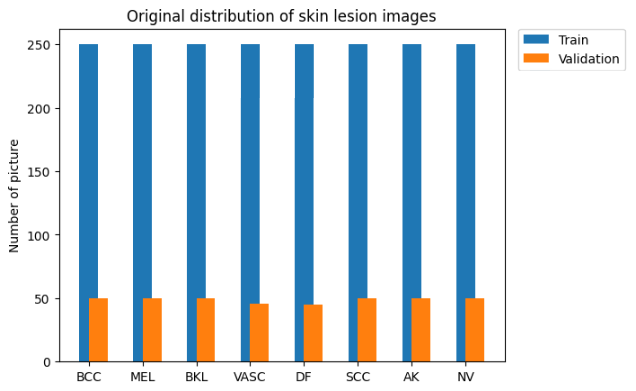
\includegraphics[scale=0.5]{images/Building/Skin lesion Balance distribution.png}
        \caption{Skin Lesions balance distribution.}
    \label{fig: Skin Lesions balance distribution}    
    \end{center}
\end{figure}

In the picture we can see the result of applying the trimming in each of the classes. The number of images to keep per class is determined by the number of minority classes.


\textbf{Step 4. Image conversion to matrix}
Since images are made up of pixels, their colours are constituted by numbers. For this work,  they are specifically represented in RGB encoding. This means that each pixel has a numerical translation ranging from 0 to 255 values. Depending on the feature extractor used, the values of the numerical matrix have to be \textbf{normalised } between 0 and 1 or between -1 and 1. 

\textbf{Step 5. Data Augmentation}

Small data sets are often used to train neural networks. This means that the network tends to \textbf{generalise} immediately due to the small variety of data. With the data augmentation technique, we generate a \textbf{series of derived images} from an original one. We have applied to them shifts, rotations, zooms, splits or changes in brightness or colour saturation to obtain new pictures. This makes the dataset richer and increases the number of images. As a demonstration of this, we have applied the transformations that we will perform on all the images in the training dataset to a random image in the figure \ref{fig: Data augmentation examples}.

\begin{figure}[ht]
    \begin{center}
        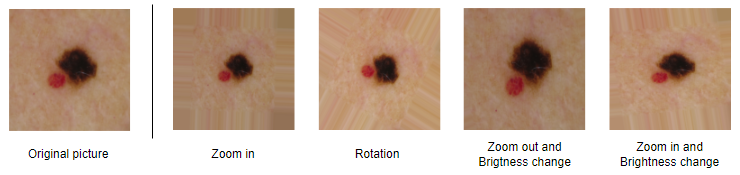
\includegraphics[scale=0.5]{images/Building/Data augmentation.png}
        \caption{Data augmentation examples.}
    \label{fig: Data augmentation examples}    
    \end{center}
\end{figure}

 

\newpage
\section{Looking for the best model}

\newpage
%% Transfer learning
\section{Transfer learning}

To achieve high metrics, it is necessary to train large data sets and long neural networks with many layers. An alternative to it is to use a pre-trained network with a very large dataset. This network has already learned to extract basic features from images efficiently. 

Have you ever seen a cartoonist working? He starts by drawing basic shapes, lines, circles, and ovals, and he composes the painting as an overlay of these shapes, adding shadows and gradients to simulate volume. The idea behind transfer learning is similar to this example. It consists on using this network in the first step as a pattern recognition layer, known as \textbf{feature extractor}. The goal of this is to extract the most informative, identifying edges, corners, blobs and extracting, at the same time, the colour histogram.  As well as, in this step is obtained a data dimensionality reduction to make it suitable for the next layer. Then the classification layer is added according to each specific categorised problem. This way, transfer learning can be applied to tasks where the dataset is not large enough to train a complete model from scratch.

Transfer learning is performed according to the following workflow:

\begin{figure}[ht]
    \begin{center}
        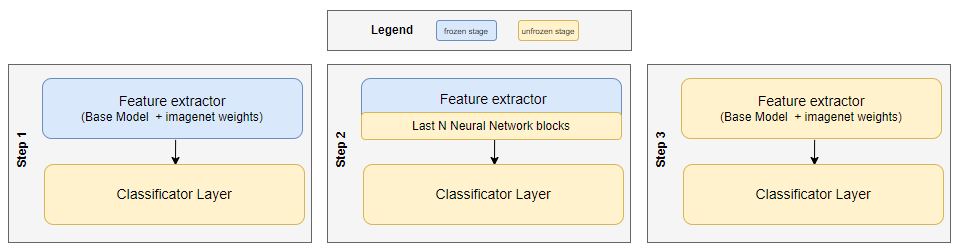
\includegraphics[scale=1.0]{images/Building/Transfer Learning phases.png}
        \caption{Transfer learning phases.}
    \label{fig: Transfer learning phases}    
    \end{center}
\end{figure}

\begin{enumerate}
    \item A\textbf{ pre-trained model}, which it will call the base model, is loaded with the training weights. This model is loaded without the classification layer (the model's top layers). The models used in this job are: \textit{Efficient B0} and \textit{ResNet 50}, both with the preloaded "\textit{imagenet}" weights. 
 
    \item Because we want to preserve its ability as a feature extractor, we \textbf{freeze all layers} of the base model.  This way we avoid destroying the information in future training rounds. Furthermore, a new set of trainable layers is added on top of the frozen layers to form the \textbf{classification layer}. The whole ensemble is trained on the dataset of skin lesion images and their weight preservers. 

    \item The next step is to load an \textbf{identical model} (extractor plus classifier) with the last block of the feature extractor unfrozen. This new network is loaded with the weights from the previous training and trained again.

    \item Finally, we perform a fine-tuning by creating a new copy of the neural network, on which we unfreeze the whole model to retrain it on the new data at \textbf{a very low learning rate}. This way, significant improvements can be achieved by gradually adapting the pre-trained features to the new data.

\end{enumerate}



\subsection{Hyper-parameters searching}

A neural network is governed by a large number of external parameters that need to be tuned to achieve network convergence.  Hyperparameter search is the process of finding the optimal set of parameters that define the model.

The parameters that will be adjusted in our work, and that are usually general to any deep learning work, are 
\begin{enumerate}
    \item \textbf{Learning Rate}: controls how much the model parameters are adjusted at each training step. A high learning rate can make the model converge quickly, but there is also a risk that the network may be lost in a global minimum and not complete learning. On the other hand, a low learning rate may lead to slow convergence or no convergence at all.

    \item \textbf{Number of Epochs}: This parameter controls the number of times the learning algorithm iterates over the entire training data set. During each epoch, the weights of the neural network are updated in an attempt to minimize the loss function, thus improving the learning process of the network for each epoch. The most common values are 16, 32 and 64, always in multiples of two.

    \item \textbf{Batch Size}: The number of training samples used in a model update iteration. Its value and the dataset size determine the number of iterations required to complete an epoch. If its value is low, the model may not have enough time to learn the patterns of the data. In contrast, a high epoch value may cause the model to be susceptible to overfitting by incorporating data noise into the weight adjustment.

    \item \textbf{The optimizer}: It is the element in charge of calculating the gradient of the cost function for each parameter/dimension of the network. It is an algorithm that tries to minimize the error function by searching for the minimum of this function. Therefore, it is a crucial element in the network learning process and its choice will determine the performance of the network. There are several down gradient optimizers in the market. In this work we have chosen two of the most used in classification works: SGD and Adam.

    \textbf{Stochastic Gradient Descent} (SGD): This optimizer limits the gradient calculation to one per batch. It is used as a baseline in order to compare the others.
    
    \textbf{Adaptative moment estimation} (Adam): It inherits and combines the improvements of the AdaGrad and RMSProp algorithms, and introduces gradient impulse averaging. The first optimizer introduces variability into the training factor concept at each iteration, unlike the SGD optimizer, which keeps it stable. The second optimizer is similar to AdaGrad but performs the training factor scaling by a different formula (the exponential decay of the square of the gradients).

    The behaviour of SDG and RMSProp optimizer can be improved using the \textit{\textbf{momentum}} parameter. This one is used to accelerate the gradient descent and dump its oscillations \cite{SGDwithMomentum}. A reference value of 0.9 is used during the hyperparameter step.

    As a complement, I add the following reference \cite{optimizers1} that shows graphically the operation of different optimizers, as well as the results of the different ones. 

    In order to find the most optimal parameters with which to train our model, we followed a \textbf{grid search} model. Thus, we set the number of \textbf{epochs to 32}, since this value is most often used as a starting point. From here we will try different combinations of learning rate and optimizers.

\end{enumerate}

\begin{figure}[ht]
    \begin{center}
        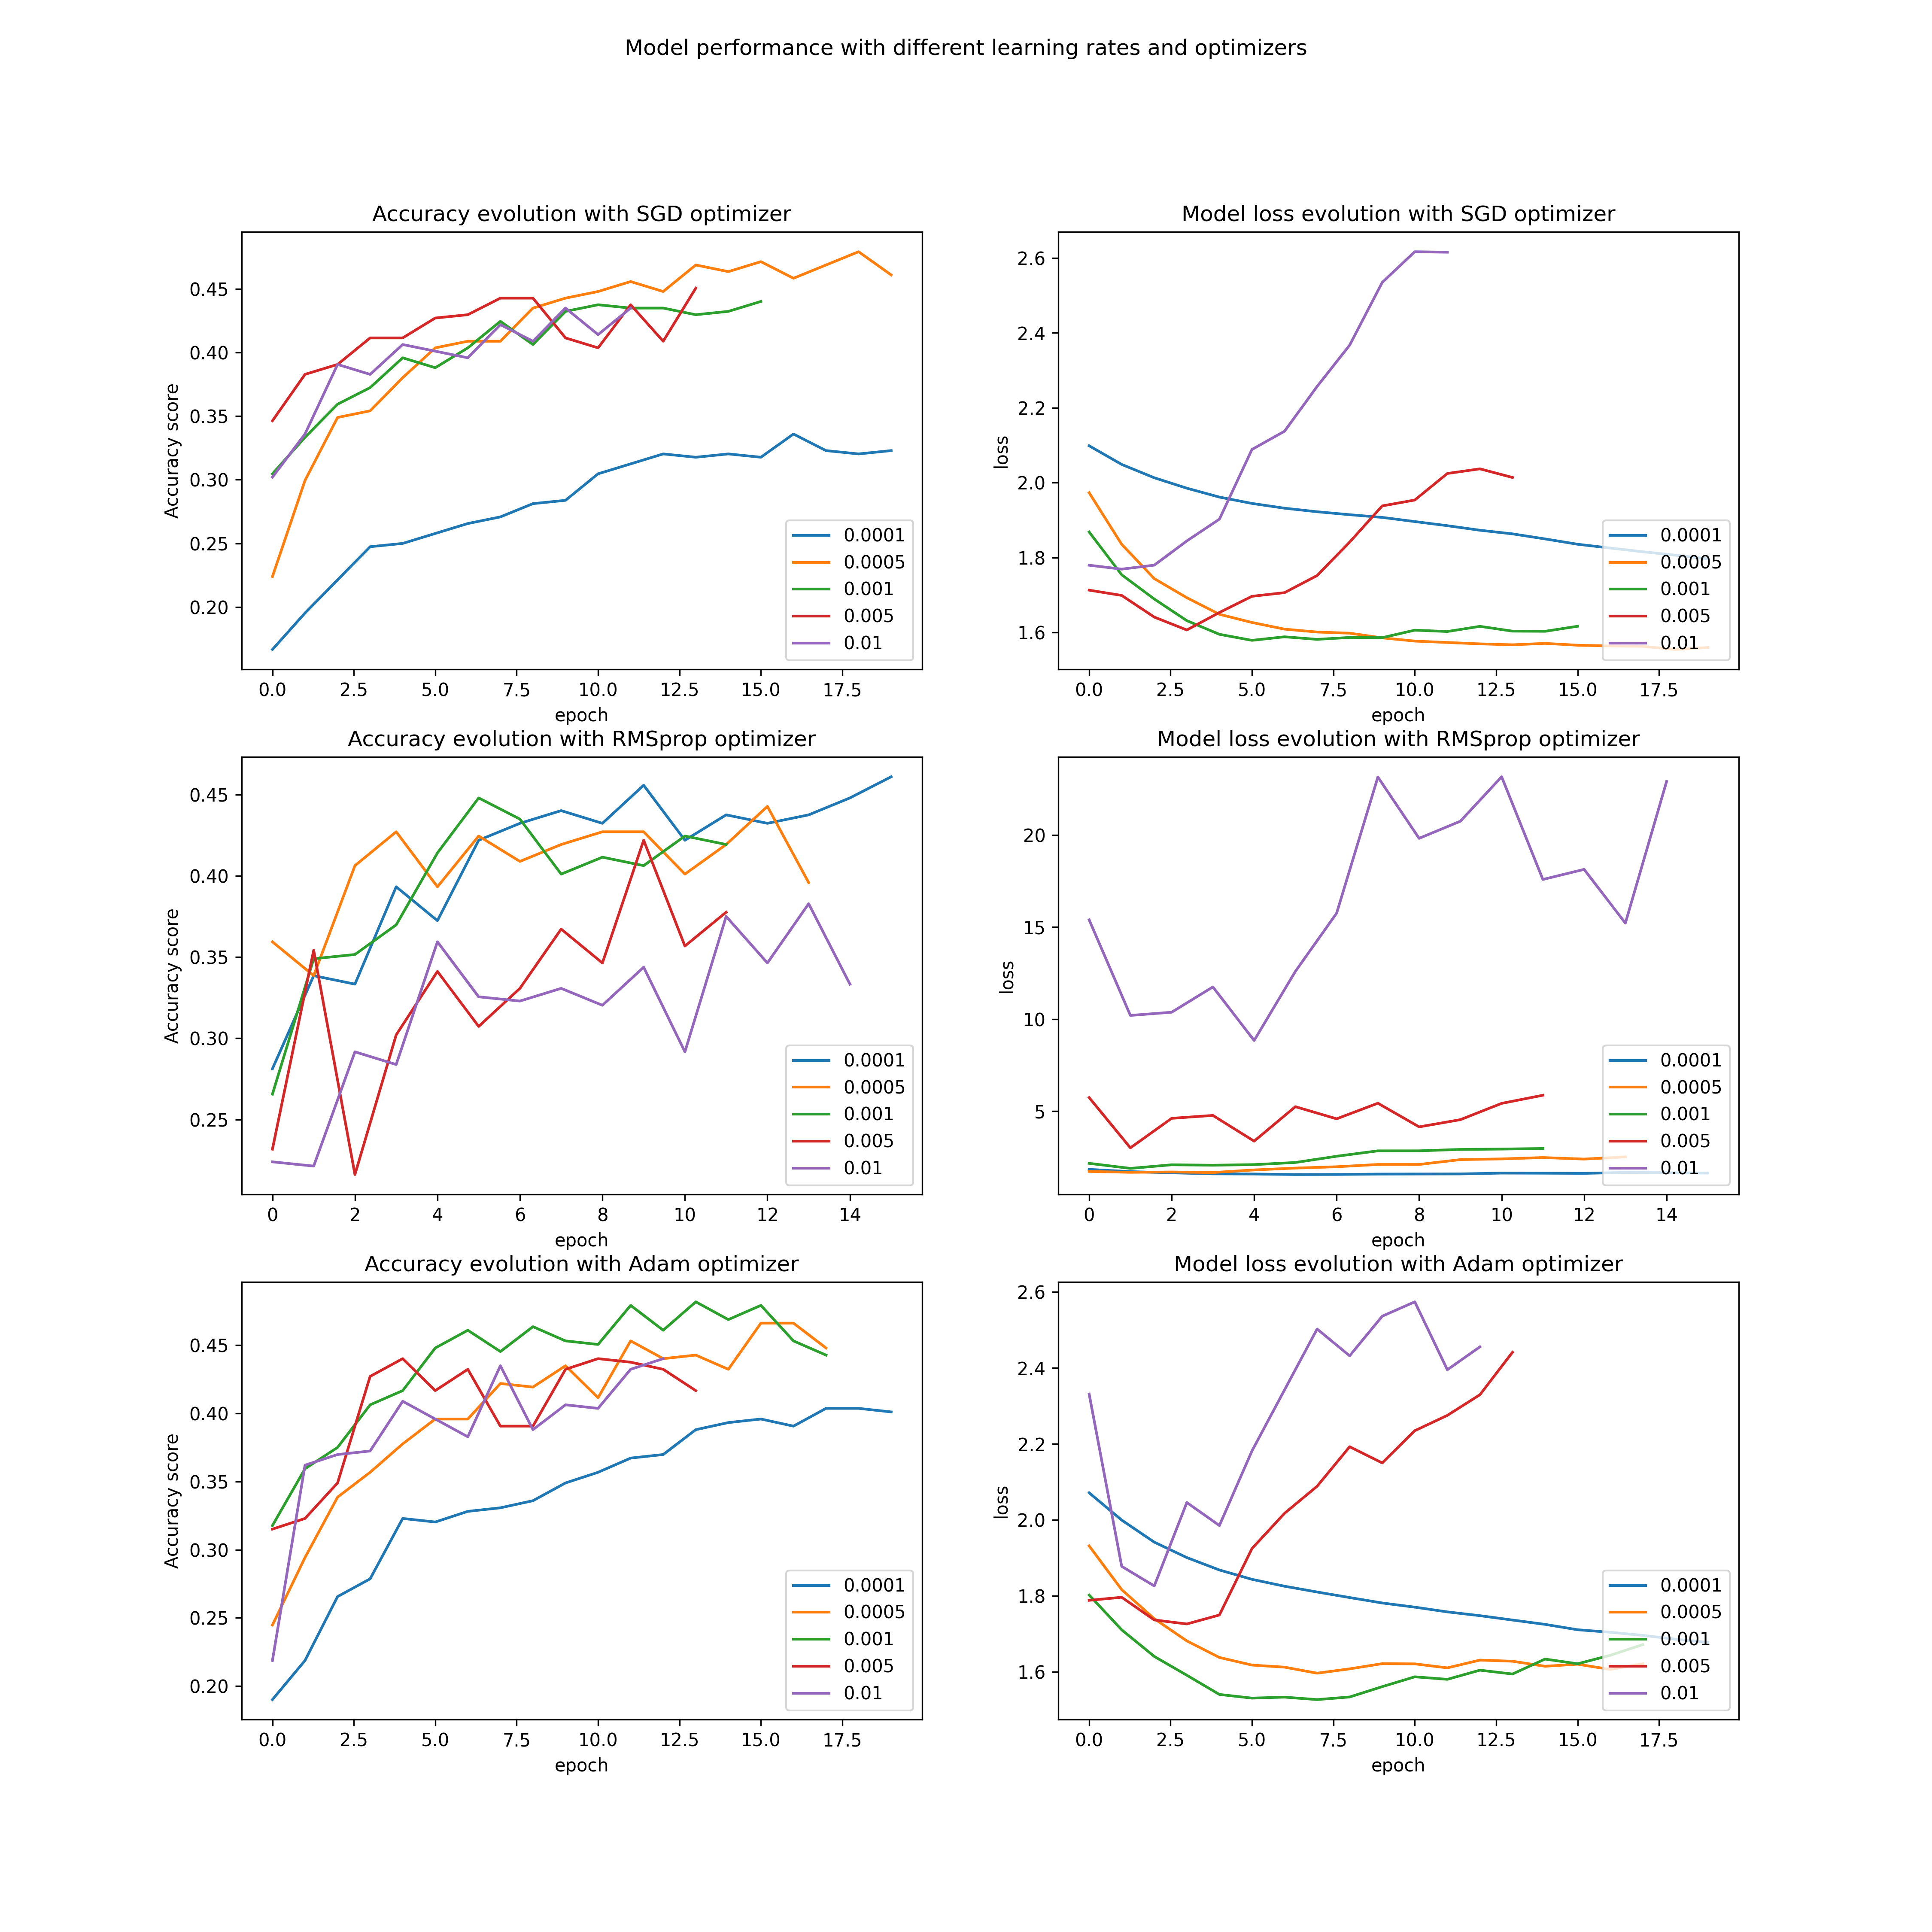
\includegraphics[scale=0.35]{images/Building/Hyperparameters/Model performance with different learning rates and optimizers.png}
        \caption{Efficient B0 base model hyperparameters searching .}
    \label{fig: EfficientB0_hyperparameters}    
    \end{center}
\end{figure}

As shown in figure \ref{fig: EfficientB0_hyperparameters}, training the model with a learning rate low value and SGD or Adam optimizer is the best combination to guarantee a smooth model convergence.  






\newpage
\subsection{Skin lesion classification with EfficientNet B0}


\subsubsection{Step 1. Base model froze}


\begin{figure}[ht]
    \begin{center}
        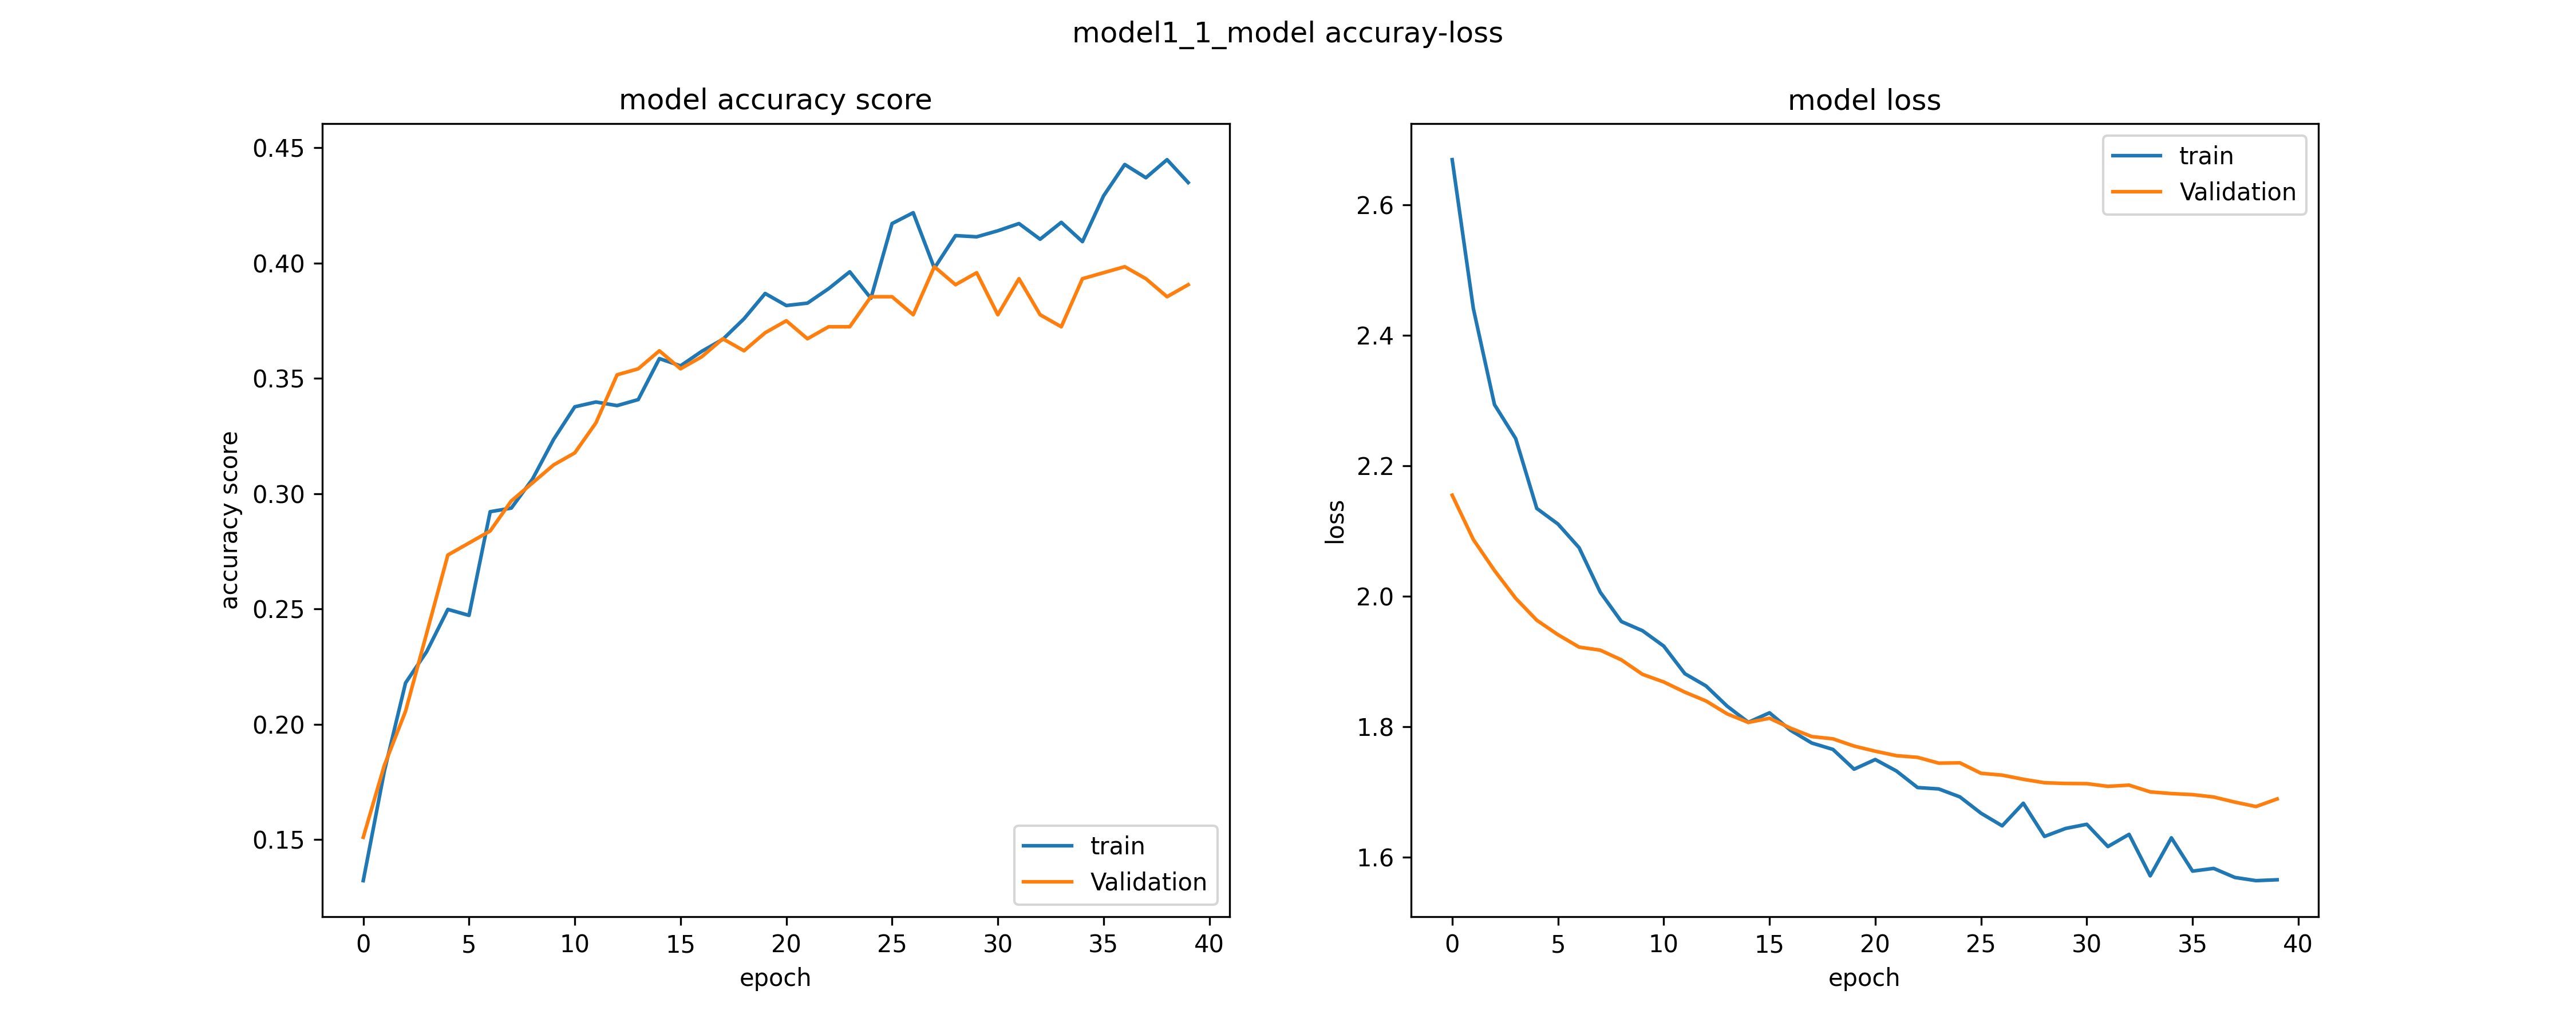
\includegraphics[scale=0.40]{images/Building/Model Efficientnet/model1_1_model accuray-loss.png}
        \caption{EfficientNet model 1. Accuracy-loss diagram.}
    \label{fig: Model1_accuracy_loss}    
    \end{center}
\end{figure}

\newpage
\subsubsection{Step 2. Unfroze Model base last block}

\subsubsection{Step 3. Unfroze the model}

\newpage
\subsection{Skin lesion classification with ResNet50}

\subsubsection{Step 1. Base model froze}

\begin{figure}[ht]
    \begin{center}
        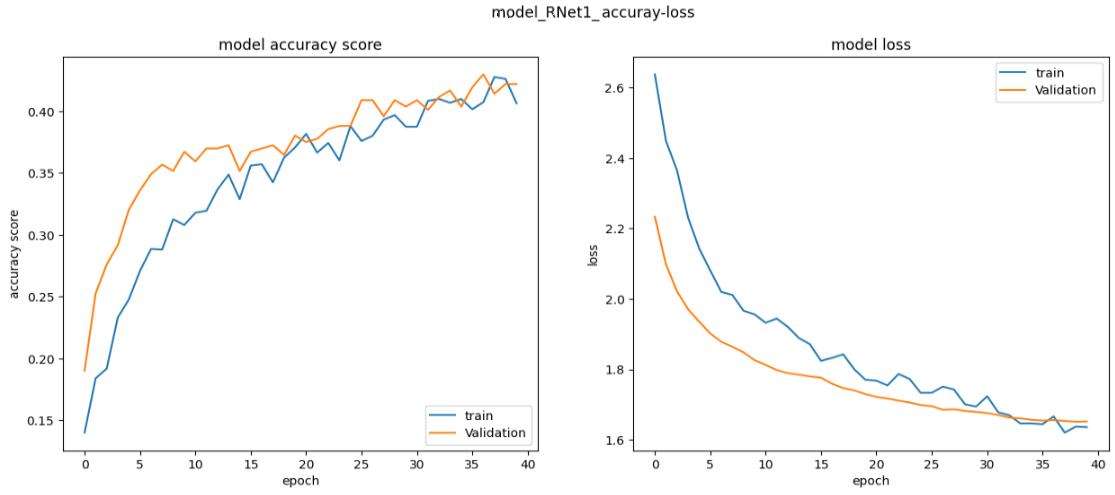
\includegraphics[scale=0.45]{images/Building/Model RestNet50/ResNet50 model accuray_loss.png}
        \caption{ResNet50 model accuracy and loss graph.}
    \label{fig: ResNet50_accuracy_loss}    
    \end{center}
\end{figure}

\subsubsection{Step 2. Unfroze Model base last block}

\subsubsection{Step 3. Unfroze the model}



